\section{实验复现}

\begin{frame}
  \frametitle{实验环境与参数设置}

\textbf{实验环境:}

RTX 3090,Pytorch 1.10.1,Python 3.7


\textbf{参数设置:}

分类任务:batchsize为24,epoch为200,学习率为0.001,optimizer为Adam

零件分割任务:batchsize为16,epoch为251,学习率为0.001,optimizer为Adam

语义分割任务:batchsize为16,epoch为32,学习率为0.001,optimizer为Adam


\end{frame}


\begin{frame}
  \frametitle{实验数据集介绍}

\textbf{ModelNet40(用于分类任务):}

包含了40个类别(如飞机,汽车等)的CAD模型数据。训练集有9843个点云数据,测试集有2468个点云数据。

\textbf{ShapeNet(用于部件分割任务):}

包含14个大类别(如飞机,椅子等)和55个小类别的CAD模型数据。训练集有14007个点云数据,测试集有2874个点云数据。

\textbf{S3DIS(用于语义分割任务):}

是大规模室内三维空间数据集,包含了6个建筑物,共计271个房间。房间内包含13类物体(如天花板、地板、门、沙发等) 。



\end{frame}


\begin{frame}
  \frametitle{数据集可视化}
\textbf{ModelNet40(分类任务):}

源数据(txt文件)进行可视化:


\begin{figure}
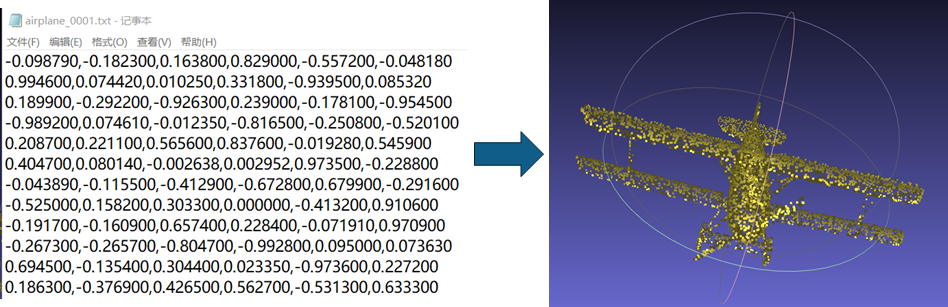
\includegraphics[scale=0.4]{doc/img/f4.png}
\end{figure}



\end{frame}



\begin{frame}
  \frametitle{数据集可视化}

\textbf{ShapeNet(部件分割任务)}

源数据(txt文件)进行可视化:


\begin{figure}
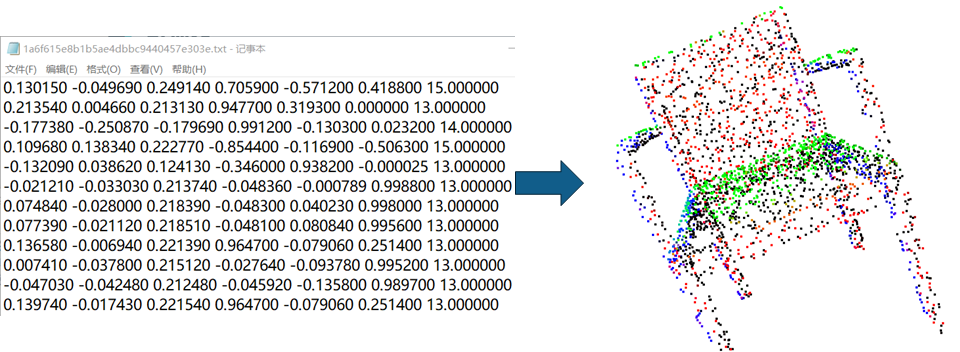
\includegraphics[scale=0.35]{doc/img/f5.png}
\end{figure}


\end{frame}


\begin{frame}
  \frametitle{数据集可视化}

\textbf{S3DIS(语义分割任务)}

源数据(txt文件)进行可视化:


\begin{figure}
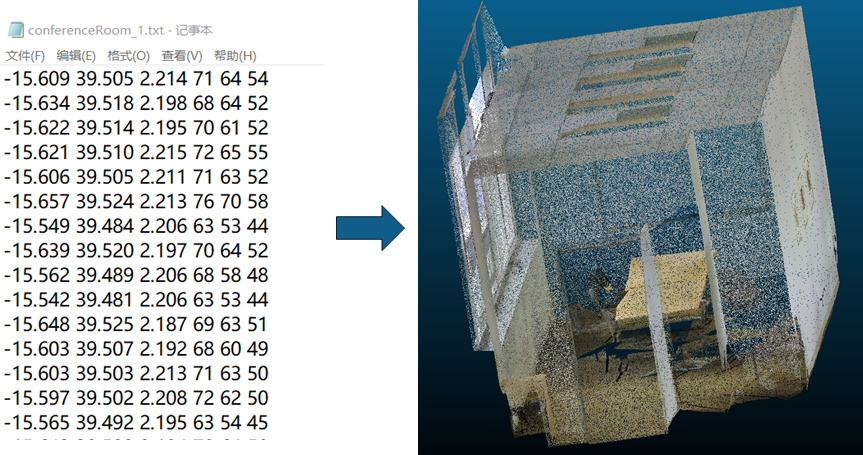
\includegraphics[scale=0.3]{doc/img/f6.png}
\end{figure}


\end{frame}


\begin{frame}
  \frametitle{实验复现结果及分析}

在ModelNet40数据集上进行分类:

\begin{figure}
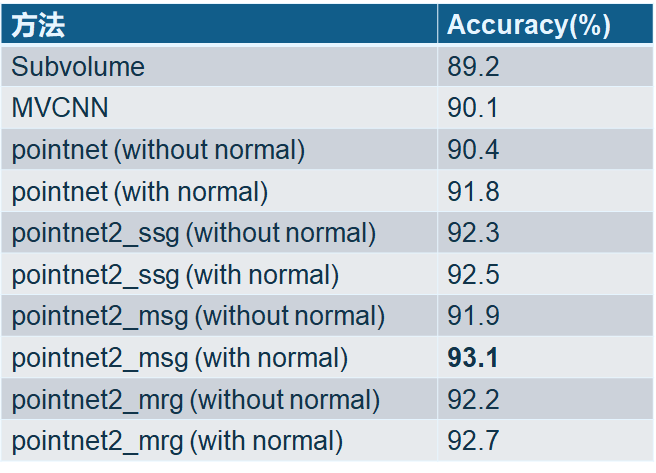
\includegraphics[scale=0.35]{doc/img/t1.png}
\end{figure}


% \begin{table}[h]
%   \centering
%   % \caption{}
%   \label{tab:q}
%   \begin{tabular}{ccccc}
%     \toprule
% 方法          & Accuracy( \% )\\
%     \midrule
% Subvolume         & 89.2 \\ \hline
% MVCNN           & 90.1 \\ \hline
% pointnet (without normal) & 90.4 \\ \hline
% pointnet (with normal) & 91.8 \\ \hline
% pointnet2\_ssg (without normal) & 92.3 \\ \hline
% pointnet2\_ssg (with normal) & 92.5 \\ \hline
% pointnet2\_msg (without normal) & 91.9 \\ \hline
% pointnet2\_msg (with normal) & 93.1 \\ \hline
% pointnet2\_mrg (without normal) & 92.2 \\ \hline
% pointnet2\_mrg (with normal) & 92.7 \\ \hline
%     \bottomrule
%   \end{tabular}
% \end{table}

\end{frame}


\begin{frame}
  \frametitle{实验复现结果及分析}

比较pointnet和pointnet++各个模型的显存占用:

\begin{figure}
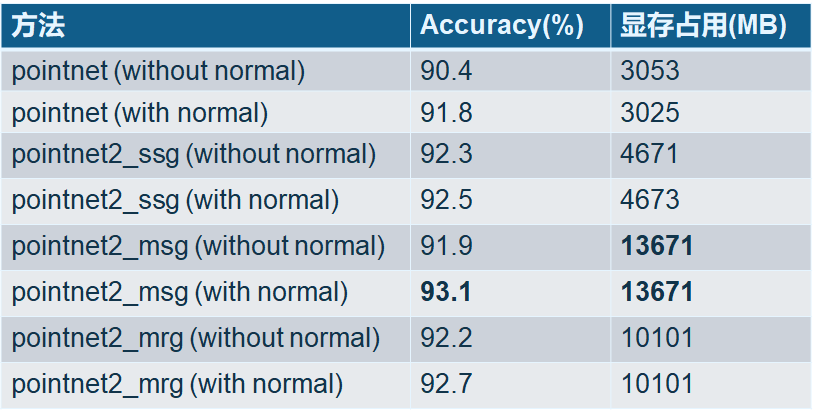
\includegraphics[scale=0.35]{doc/img/t2.png}
\end{figure}



\end{frame}



\begin{frame}
  \frametitle{实验复现结果及分析}

在ShapeNet数据集上进行部件分割:

\begin{figure}
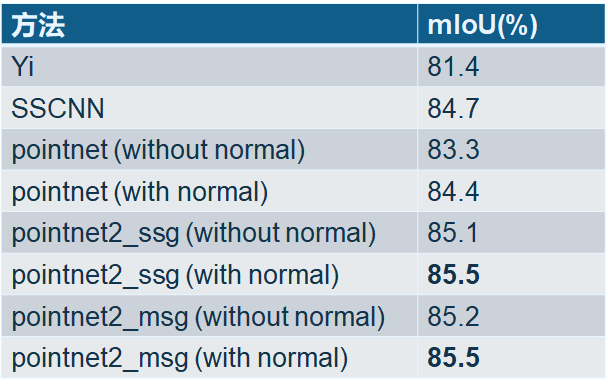
\includegraphics[scale=0.35]{doc/img/t3.png}
\end{figure}


\end{frame}

\begin{frame}
  \frametitle{实验复现结果及分析}

在S3DIS数据集上进行语义分割:


\begin{figure}
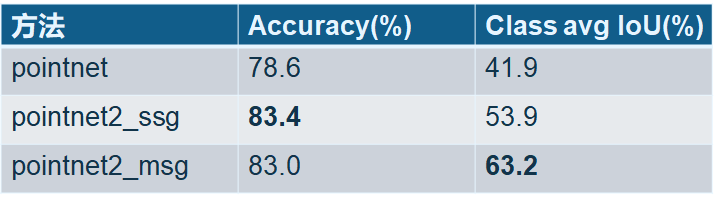
\includegraphics[scale=0.35]{doc/img/t4.png}
\end{figure}

\end{frame}


\begin{frame}
  \frametitle{S3DIS语义分割结果可视化}

\begin{figure}
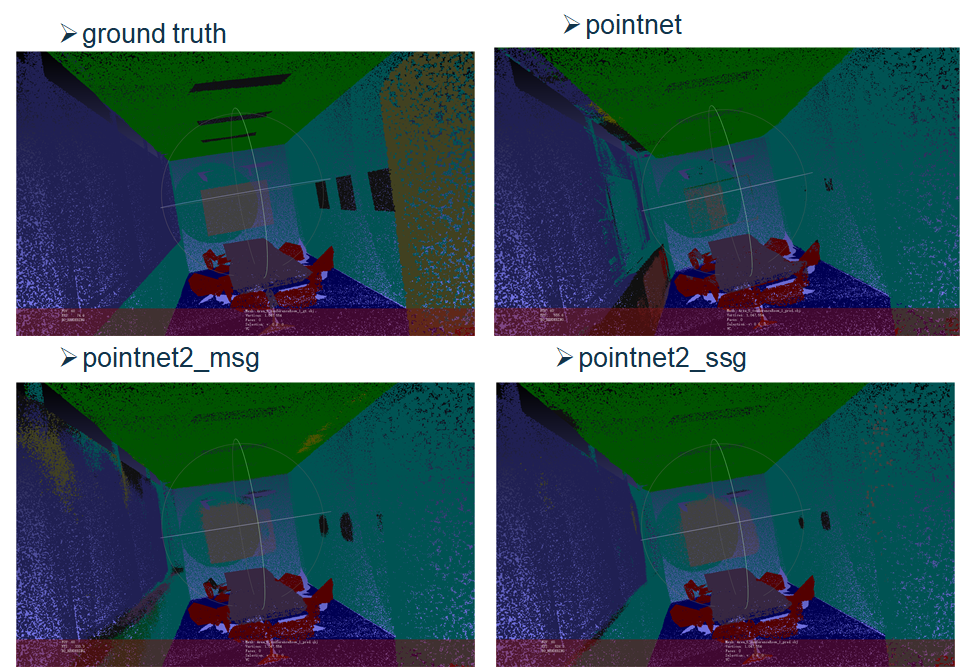
\includegraphics[scale=0.3]{doc/img/f7.png}
\end{figure}


\end{frame}

